\documentclass[12pt, a4paper]{scrreprt}

\renewcommand*\familydefault{\sfdefault} 
%\usepackage[T1]{fontenc}

\usepackage[english]{babel}
%\usepackage{cite}
\usepackage[utf8]{inputenc}
%\usepackage[onehalfspacing]{setspace}
\usepackage{geometry, textcomp}
\newgeometry{right=2cm,left=4cm, top=2.5cm, bottom=2.3cm, footnotesep=0.5cm}
%\usepackage[acronym]{glossaries}

\usepackage[printonlyused]{acronym}  % Abkürzungsverzeichnis [nur verwendete Abkürzugen]

%\glsenablehyper

%\makeglossaries

\usepackage{savesym}
\usepackage{amsmath,amssymb,amstext}
%\usepackage{graphics}
\savesymbol{iint}
\usepackage{txfonts}

\restoresymbol{TXF}{iint}
\usepackage[automark,headsepline,ilines,komastyle]{scrpage2}
\usepackage{blindtext}
\usepackage[euler]{textgreek}
\setlength{\parindent}{0pt}
\setlength{\headheight}{1.5\baselineskip}
\renewcommand{\baselinestretch}{1.5}

\pagestyle{scrheadings}
\clearscrheadfoot
\ihead[]{}
\chead[]{}
\ohead[]{\headmark \hfill \thepage}
\ifoot[]{}
\cfoot[]{}
\ofoot[]{}

\setheadsepline[\textwidth]{1pt}
\usepackage{tabularx}
\usepackage{colortbl}
\usepackage{multirow}
\usepackage{hhline}
\usepackage{array}
\usepackage{tocloft}
\usepackage[hidelinks]{hyperref}
\tocloftpagestyle{scrheadings}
\renewcommand{\chapterpagestyle}{scrheadings}
\usepackage[font=footnotesize]{caption}

\usepackage{tikz}
\usepackage{rotating} 

\newenvironment{packed_item}
	{\begin{itemize}
			\setlength{\itemsep}{0pt}
			\setlength{\topsep}{0pt}
			\setlength{\parsep}{0pt}
			\setlength{\parskip}{0pt}}
		{\end{itemize}}
	
\usepackage[style=authoryear, natbib=true, backend=biber]{biblatex}

\renewcommand{\nameyeardelim}{ }
\usepackage[babel,german=guillemets]{csquotes}

\makeatletter

\newrobustcmd*{\parentexttrack}[1]{%
	\begingroup
	\blx@blxinit
	\blx@setsfcodes
	\blx@bibopenparen#1\blx@bibcloseparen
	\endgroup}

\AtEveryCite{%
	\let\parentext=\parentexttrack%
	\let\bibopenparen=\bibopenbracket%
	\let\bibcloseparen=\bibclosebracket}

\makeatother

\usepackage{pstricks}
\usepackage{pstricks-add}

\bibliography{Lit.bib}

\usepackage[final]{pdfpages}

\begin{document}
		\begin{titlepage}
			\begin{center}
			%\setlength{\headheight}{1.5\baselineskip}
			\renewcommand{\baselinestretch}{1.5}
					\textbf{\large FOM - Hochschule für Oekonomie \& Management \\
						Hamburg \\
						\ \\
						Master-Studiengang Big Data \& Business Analytics \\
						3. Semester \\
						\ \\
						Development of a system to control and monitor blood pressure \ \\
						measurements to prevent cardiovascular disease \ \\
						\ \\
						}
						
					\textrm{
						\ \\
						Betreuer: Prof. Dr. Kai Brüssau \\
						\ \\
						Autor: Jacqueline Franßen \\
						\ \\
						Matrikel-Nr: 496804 \\
						\ \\
						3. Fachsemester \\
						\ \\
						Hamburg, den 29.02.2020 \\
						}
			\end{center}
		\end{titlepage}

%\includepdf{Image/Deckblatt.pdf}

			\setcounter{tocdepth}{3}
			\setcounter{secnumdepth}{3}		
			\pagenumbering{Roman}
			\thispagestyle{empty}
			\pdfbookmark{\contentsname}{toc}\tableofcontents
			\newpage
			\listoffigures
			\listoftables

			\pagenumbering{arabic}
			\thispagestyle{empty}
\chapter{Abstract}\label{abstract}

This thesis tackles the problem of automated detection of inconsistencies in evolving knowledge graphs, which arise from periodic updates that affect graph elements connected to unchanged elements.
The proposed inconsistency detection approach is developed based on the analysis of a knowledge graph from the medical coding domain which is subject to annual updates. To assess the effectiveness and efficiency of the approach, two experiments based on real- world and synthetically generated data are conducted. Three graph versioning approaches are taken into consideration for the analysis of their impact on the effectiveness and efficiency of the inconsistency detection approach. The experimental results showed that inconsistency detection can be automated by analyzing subgraphs, containing elements whose change constitutes an inconsistency source, with respect to the alteration of its elements by a periodic update. The effectiveness and efficiency of the approach depend on the graph versioning approach, the primary change type (deletion, addition, or update) and the number of inconsistency-causing changes.
This work provides an approach that facilitates targeted graph corrections and incremental updates instead of graph reconstructions by enabling cross-state graph verification without the need for a large graph-underlying data set.

only documentation of blood pressure values, not measurement (current hardware of smartphone not able)

- how can diagrams be displayed on smartphones? --> only show a certain part of data

\chapter{Abbreviations}
\begin{acronym}[CRISP-DM]
\acro{crisp-dm}[CRISP-DM]{CRoss-Industry Standard Process for Data Mining}
\acro{cfo}[CFO]{Chief Financial Officer}
\acro{who}[WHO]{World Health Organization}
\acro{iarc}[IARC]{International Agency for Research on Cancer}
\acro{ham10000}[HAM10000]{Human Against Machine with 10000 training images}
\end{acronym}

% 01 introduction
\chapter{Introduction}\label{introduction}

\section{Problem statement}
\section{Aim and scope of this work}

%describe aim
The first aim of this scientific work is to develop a solution ...
%describe scope
What is important, the developed model is only a reference model....


% 02 related work
\chapter{Related Work}\label{relatedwork}


example architecture

Deep learning methods use multiple layers of nonlinear processing units for feature extraction and transformation and to find deep relationships between complex variations under supervised and unsupervised procedures.


% 03 theoretical background
\chapter{Theoretical Background for Problem Context}\label{background}
\section{\ac{crisp-dm}: Standard Process for Data Mining projects}


% 04 development 
\chapter{Development of an architectural design to analyze data sources from healthcare providers}


% 05 experimental evaluation
\chapter{Experimental evaluation of architectural design}

% 06 Discussion
\chapter{Discussion}

% 07 Conclusion
\chapter{Conclusion}




\printbibliography[heading=bibintoc]

\chapter{Appendix A}\label{appendix a}
\ohead[]{Ehrenwörtliche Erklärung \hfill \thepage}

\null\vfill
\textbf{Ehrenwörtliche Erklärung}

Hiermit versichere ich, dass die vorliegende Arbeit von mir selbstständig und ohne unerlaubte Hilfe angefertigt worden ist, insbesondere dass ich alle Stellen, die wörtlich oder annähernd wörtlich aus Veröffentlichungen entnommen sind, durch Zitate als solche gekennzeichnet habe. Ich versichere auch, dass die von mir eingereichte schriftliche Version mit der digitalen Version übereinstimmt. Weiterhin erkläre ich, dass die Arbeit in gleicher oder ähnlicher Form noch keiner Prüfungsbehörde / Prüfungsstelle vorgelegen hat. Ich erkläre mich damit nicht einverstanden, dass die Arbeit der Öffentlichkeit zugänglich gemacht wird. Ich erkläre mich damit einverstanden, dass die Digitalversion dieser Arbeit zwecks Plagiatsprüfung auf die Server externer Anbieter hochgeladen werden darf. Die Plagiatsprüfung stellt keine Zurverfügungstellung für die Öffentlichkeit dar.

\ \\ \ \\ 


Ort, Datum (Vorname Nachname)

\vfill
%\chapter{Appendix B}\label{appendix b}
%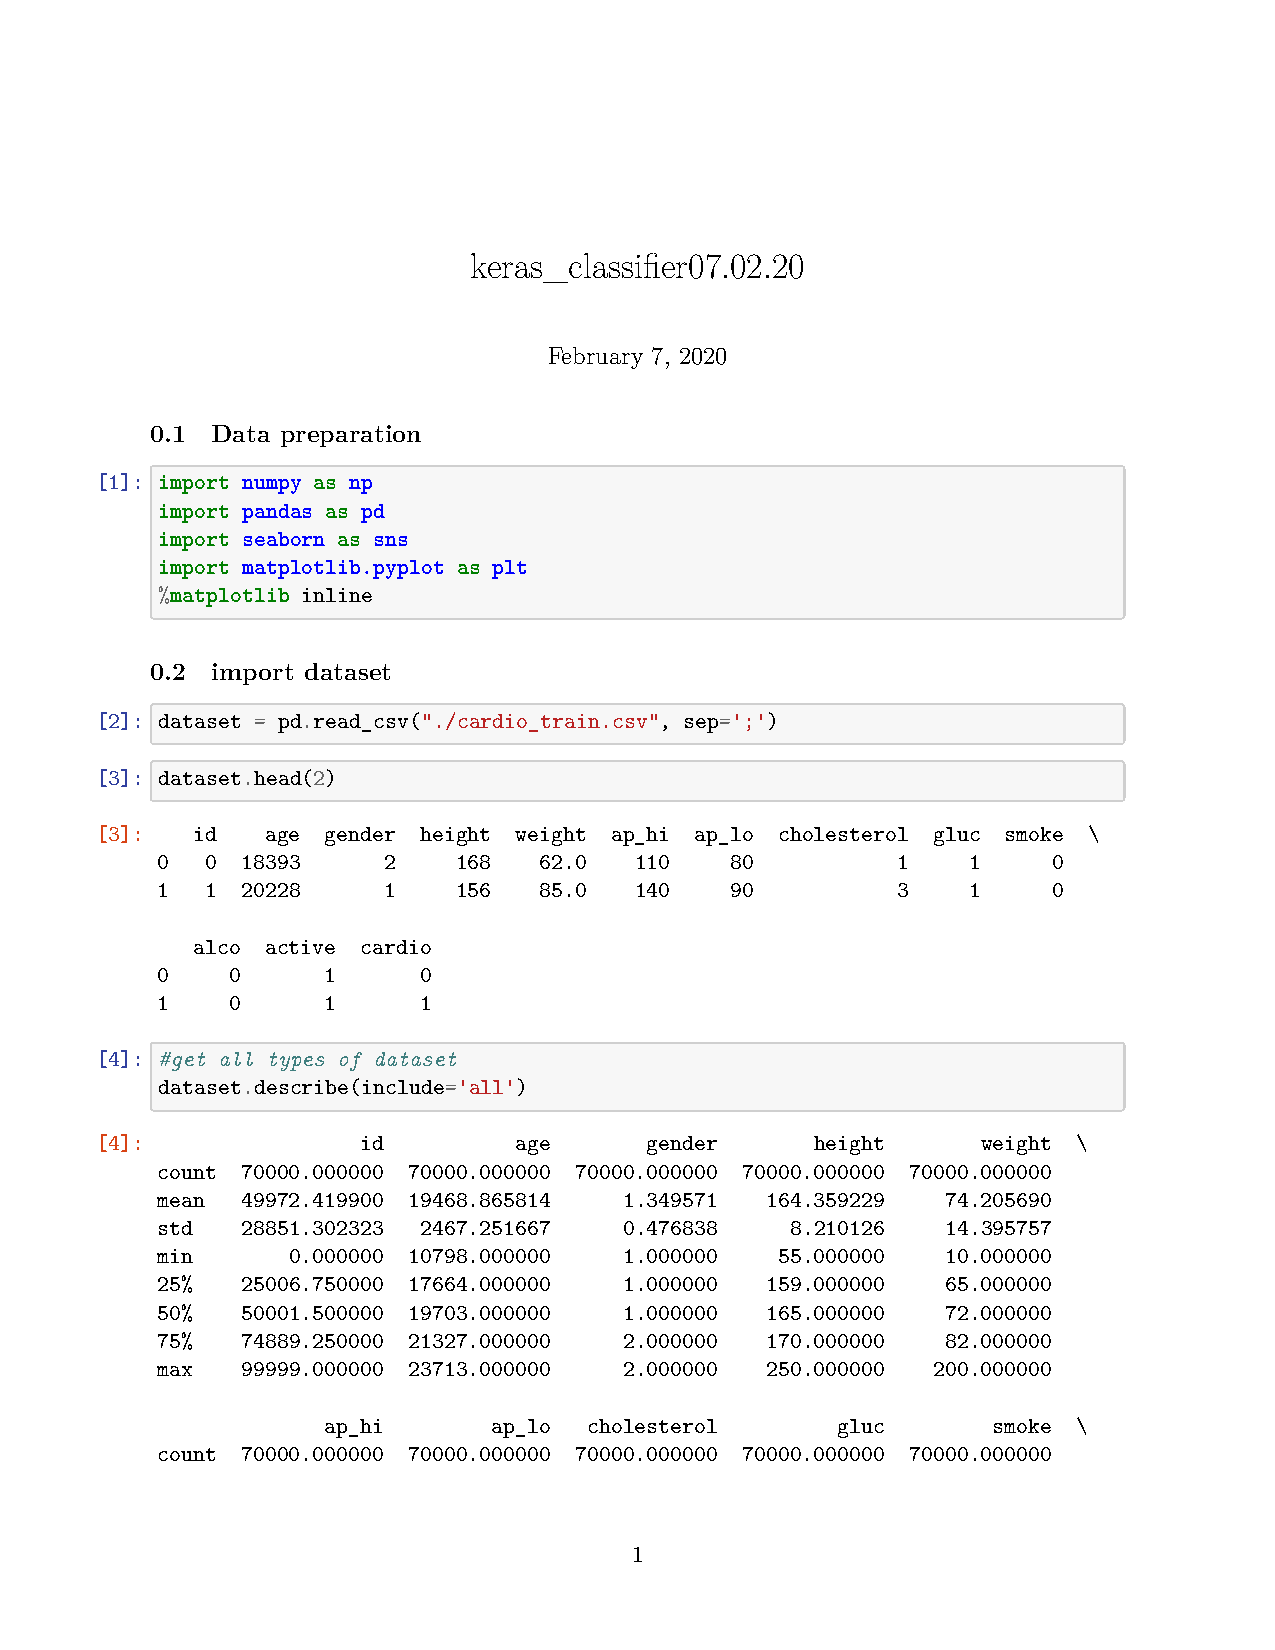
\includepdf[pages=-]{keras_classifier.pdf}

\end{document}
